\section{Comment structurer le projet ?}
Le projet consiste à développer un jeu inspiré de Tron, où plusieurs joueurs contrôlent des motos lumineuses qui laissent un mur derrière elles. Le but est d'éviter de percuter un mur placé par une autre joueur ou sois même, tout en tentant de piéger les adversaires. Ce projet nécessitera la mise en place d’une logique de jeu fluide ainsi qu’un rendu graphique performant.

\subsection{Le jeu de Tron}
Pour concrétiser le jeu en code, nous avons adopté une approche modulaire en représentant le plateau sous forme d’une \textbf{grille}, où chaque case peut contenir différents types d’entités. Les principales entités du jeu incluent les \textbf{murs}, qui définissent les limites et les obstacles, ainsi que les \textbf{joueurs}, qui se déplacent tour par tour en fonction d’un \textbf{algorithme de décision} qui leur est assigné.
Chaque joueur suit un algorithme spécifique qui détermine sa prochaine action en fonction de l’état actuel de la grille. Cet algorithme permet comme MAXN ou Paranoid d’anticiper les mouvements adverses. À chaque tour, les joueurs exécutent leur algorithme, choisissent une direction, et mettent à jour la grille en conséquence. Le jeu se poursuit jusqu’à ce qu’il ne reste plus qu’un seul joueur en vie ou qu’une condition de fin soit atteinte.
Ce modèle permet une grande flexibilité : il est facile d’expérimenter avec différents algorithmes d’IA en remplaçant simplement l’algorithme de décision d’un joueur, sans modifier la structure générale du jeu.

\subsection{Choix technologiques}
Pour réaliser ce projet, plusieurs technologies ont été sélectionnées afin d’assurer un bon équilibre entre performance, rendu graphique et analyse des parties jouées :
\begin{itemize}
    \item \textbf{C++} : Nous avons choisi C++ car, après avoir largement travaillé avec Java et Python durant nos trois années de licence, nous souhaitions explorer un langage plus bas niveau, réputé pour sa rapidité et son efficacité. C’était également un challenge intéressant qui nous permettait de mieux comprendre la gestion fine de la mémoire et d’optimiser les performances du jeu.
    \item \textbf{CMake} : CMake a été choisi pour sa capacité à gérer la compilation de manière efficace et à s’adapter à différents environnements de développement. Cela nous a permis de simplifier le processus de construction du projet et d’assurer une portabilité entre différentes plateformes.
	\item \textbf{DirectX 11} : Nous avons décidé d’utiliser DirectX 11 afin d’éviter les bibliothèques graphiques intermédiaires et travailler directement à un niveau plus bas pour mieux maîtriser le rendu. Cette approche nous a permis d’avoir un contrôle total sur l’affichage, d’assurer un rendu fluide et optimisé, et d’explorer en profondeur le fonctionnement d’un moteur graphique minimaliste.
    \item \textbf{Multithreading} : Le multithreading a été utilisé pour améliorer la fluidité et l’efficacité du jeu. Nous avons séparé le calcul des algorithmes des joueurs du moteur de jeu lui-même afin d’éviter les blocages et d’assurer une exécution réactive. De plus, nous avons intégré le multithreading dans DirectX 11 pour afficher un écran de chargement pendant que les indices et vertices du jeu sont calculés, améliorant ainsi l’expérience utilisateur.
    \item \textbf{React} : Nous avons utilisé React pour créer une interface web permettant d’afficher et d’analyser les statistiques des parties. Cela inclut le suivi détaillé des actions des joueurs, la visualisation des décisions prises à chaque tour, ainsi que l’exploitation des données sous forme de graphiques et d’indicateurs pertinents. React nous a semblé être un choix pertinent pour présenter ces informations de manière claire, interactive et esthétique.
	\item \textbf{Double Git}: Pour pouvoir profiter pleinement de ce projet pour notre avenir, nous avons mis en place un double git afin de mettre le projet non seulement sur la forge pour le rendu de l’UE, mais aussi sur Github pour pouvoir garder ce projet et ses commits de notre côté après la fin de l’année.
\end{itemize}
Cette combinaison de technologies nous a permis d’optimiser à la fois les performances du jeu, la gestion des calculs et l’analyse des résultats, tout en relevant un défi technique stimulant.

\subsection{Présentation de l'architecture du projet}
Représentation du projet via les packages et fichiers principaux.

\subsubsection{Exécuter le jeu}
\begin{figure}[h]
	\centering
	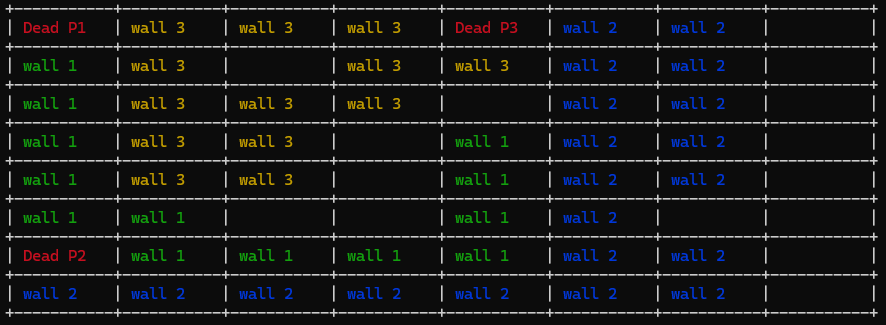
\includegraphics[width=0.9\textwidth]{images/ConsoleGame.png}
	\caption{visualisation du jeu en console}
	\label{ConsoleGame}
\end{figure}
Notre projet offre deux modes d'exécution : une \textbf{visualisation en console} et un affichage graphique avec DirectX. La version console permet de suivre facilement le déroulement du jeu avec une représentation claire des murs et des positions des joueurs, offrant une compréhension rapide de l’état de la partie en temps réel. \\
Pour personnaliser les conditions de jeu, nous avons intégré un fichier \textbf{config.ini} à la racine du projet. Ce fichier permet d'ajuster différents paramètres comme la taille de la grille, le nombre de joueurs, l’algorithme utilisé, ou encore des options plus spécifiques comme l’activation du spawn aléatoire des joueurs et la profondeur d’exploration des algorithmes. Grâce à cette approche, nous pouvons tester rapidement différentes configurations sans modifier directement le code source.

\subsubsection{Représentation avec Gource}
\begin{figure}[h]
	\centering
	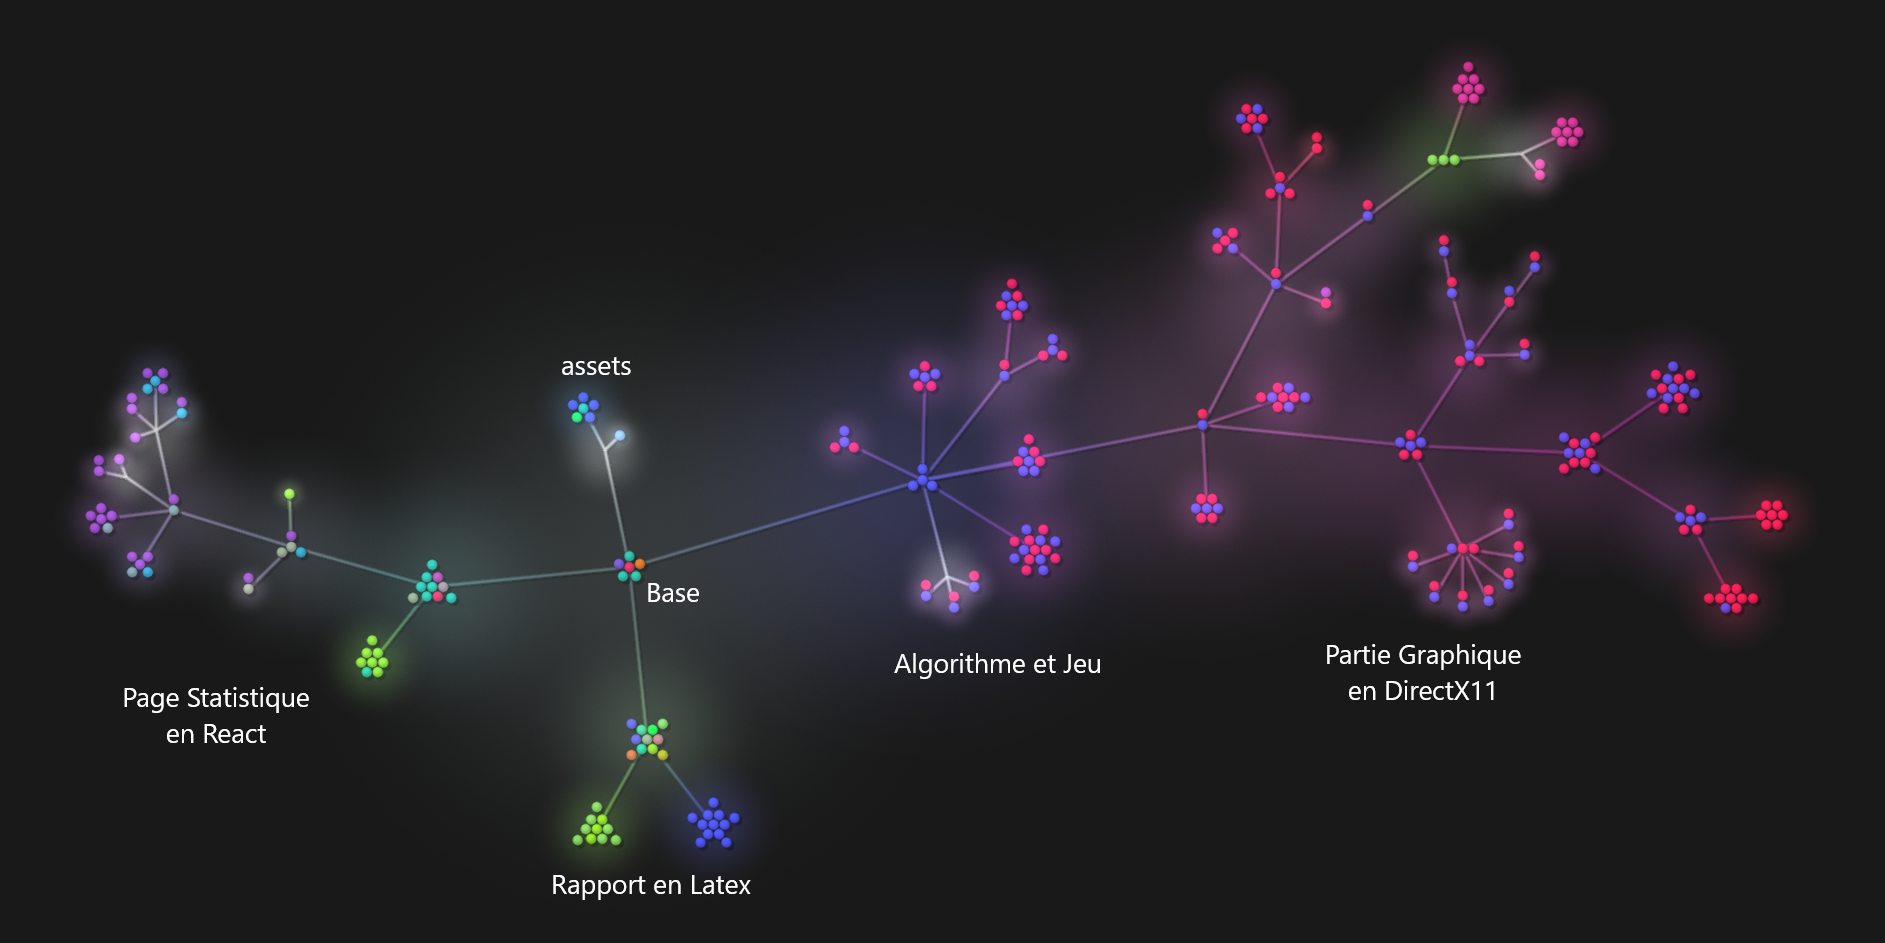
\includegraphics[width=1.0\textwidth]{images/GourceScreenFinal.png}
	\caption{Représentation du projet avec Gource}
	\label{GourceScreen}
\end{figure}
Juste ci-dessus on peut voir une représentation du projet avec Gource, qui nous permet de percevoir tous les fichiers sous formes de bulles. A la base du projet on peut voir les fichier de configuration tel que le CMakeLists, le README etc… sur la droite on peut voir le /src avec les dossiers principaux tels que les managers, les algos, etc.. Si on continue on peut voir toute la partie graphique avec tout ses sous dossier qui occupe une grande partie du projet. Si on revient sur la gauche on peut voir toute la partie de la page en react qui nous sert à voir les résultats de nos algorithmes.

\newpage

\subsubsection{Structure plus précise}
\begin{wrapfigure}{l}{0.6\textwidth}
	\centering
	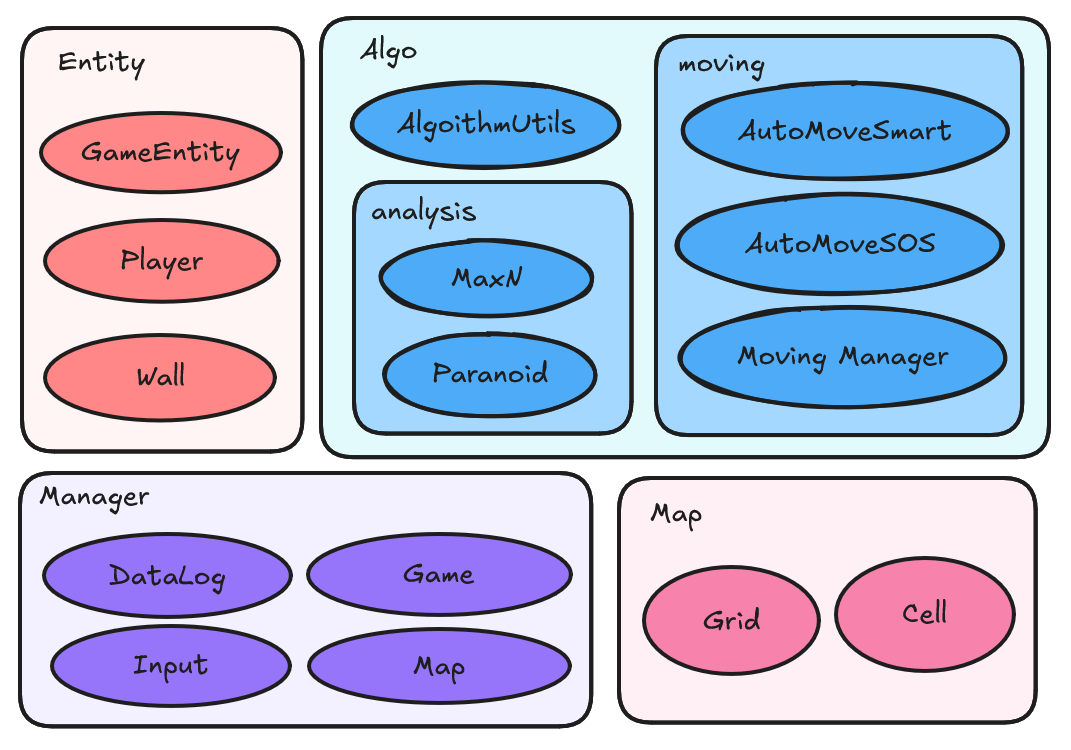
\includegraphics[width=0.6\textwidth]{images/ExcalidrawBase.png}
\end{wrapfigure}

\fbox{Diagramme de la base} \\ \\
Juste ici on peut voir une structure plus détaillée de la structure de base du jeu avec les fichier associée par package principaux. \\
Les managers vont relier ces fichiers ensemble pour faire le jeu et envoyer les résultats à la page web. \\ \\ \\ \\

\begin{figure}[h]
	\centering
	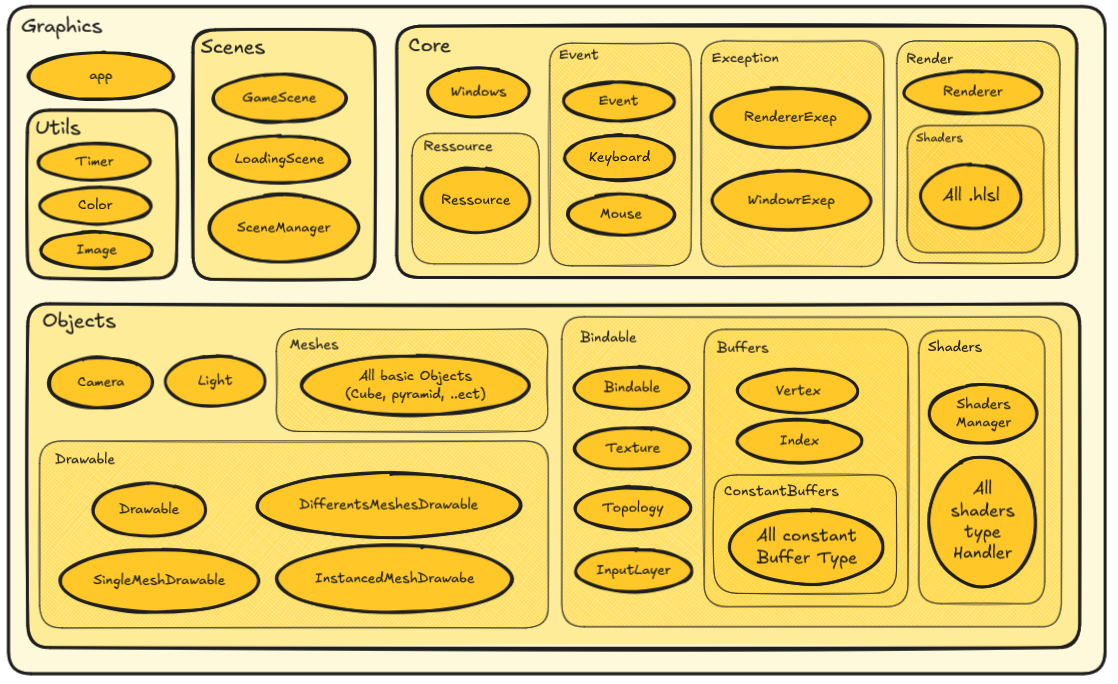
\includegraphics[width=0.9\textwidth]{images/ExcalidrawGraphics.png}
	\label{ExcalidrawGraphics}
	\caption{Représentation du projet par fichier et package important}
\end{figure}

Juste au dessus de ça on peut voir une structure plus détaillée mais toujours simplifiée pour ne montrer que les fichier et package important de la partie graphique. 
On détaillera son fonctionnement dans la partie suivante, mais cela permet de se représenter que la cette partie nous a pris plus de ressource que prévu et représente une partie importante du projet.



